\documentclass{article}

\usepackage{tikz}

\begin{document}

\begin{center}
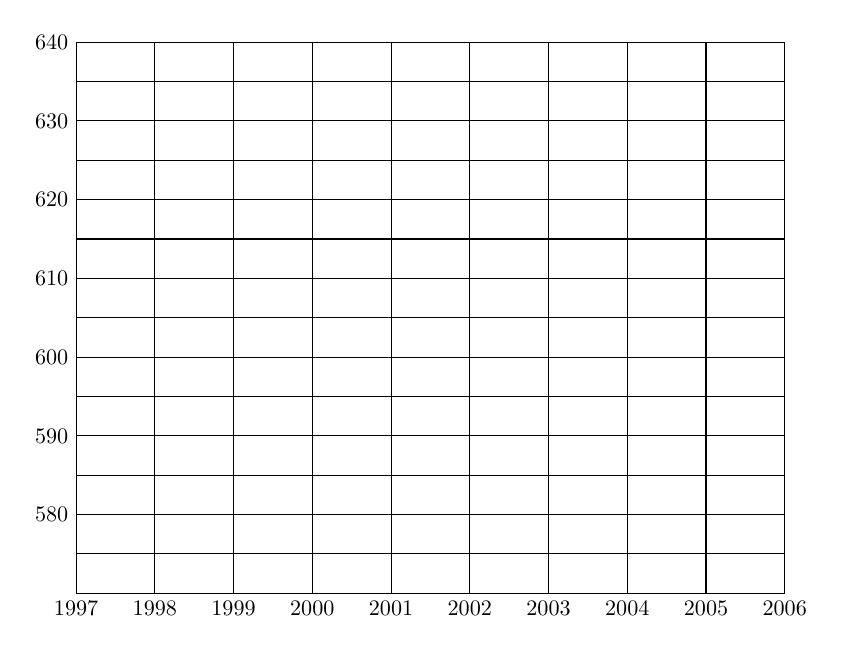
\begin{tikzpicture}
	\draw (7,57) grid [ystep=5.00001mm] (16,64);
	\draw[thick] plot[mark=ball,mark size=4pt] file {producRiz.txt};

	\foreach \x in {1997,1998,...,2006}
		\draw (\x-1990,57) node [below,scale=0.8]{\x};

	\foreach \y in {58,59,...,64}
		\draw (7,\y) node[left,scale=0.8]{\y0};
\end{tikzpicture}

Production annuelle mondiale de riz en million de tonnes
\end{center}

\end{document}
